\subsection{System architecture and  device connection scheme}
\label{sec:device_connection_scheme}
Devices in a system may be interconnected in various ways.
Some embedded systems \textbf{do not have} any connections at all. 
Such systems only sense or control the environment and there is no need to
send data somewhere. These are usually highly embedded devices with limited
amount of functions (alarm display controller, microwave or washing machine
controller).

Another group of devices are systems that are able to interchange
information using \textbf{proprietary} communication methods at \textbf{physical
and logical} layers. These systems can send information to another systems, but
they are using non standard protocols for data transmission.

Third group uses standard (serial line, ethernet with ip protocol)
communication techniques at the physical and transport level and some \textbf{proprietary
logical} protocol above that.

Last group can integrate with all other systems and has \textbf{full
communication} possibilities. These systems use standard application protocols
and transfer data over well known channels.

Research paper ~\cite{lws_milanovic.pdf} introduces three architectures , that
cover three possible ways of connectivity between devices in previously 
mentioned groups: proxy, translator and full architecture.



\begin{figure}[H]
        \centering		  
		  
		\subfloat[Proxy approach provides physical and logical conversion]{
			\label{fig:proxy_arch}
			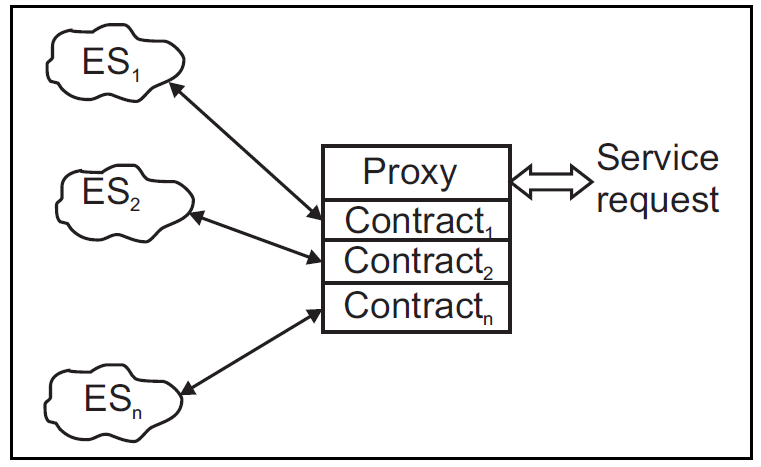
\includegraphics[width=0.3\textwidth]{../images/implementation/proxy_arch.png}
		} 
		\subfloat[Translator approach provides logical conversion]{
			\label{fig:tranlator_arch}
			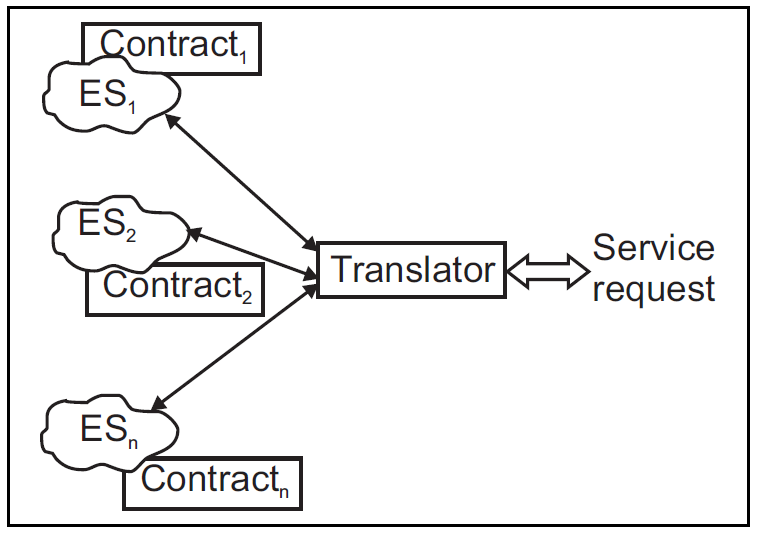
\includegraphics[width=0.3\textwidth]{../images/implementation/translator_arch.png}
		}
		\subfloat[Full approach where embedded systems directly provide services for the environment]{
			\label{fig:full_arch}
			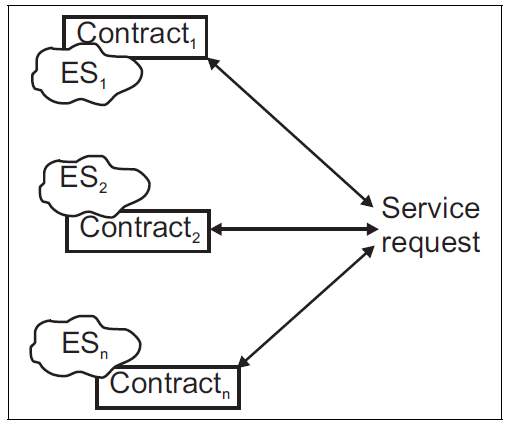
\includegraphics[width=0.3\textwidth]{../images/implementation/full_arch.png}
		} 
		       
        \caption{Possible connection architectures for the embedded services}
        \label{fig:connection_architectures}
\end{figure}




Proxy is a device which is between the client and the embedded service. It
provides services to the client and in the same time can communicate with
embedded system using closed protocols. Proxy device stores service contracts
onboard and know all specifications of connected embedded systems. 

Translator approach is similar to the Proxy, but it covers devices with proprietary
logical communication. The underlying physical transport is common to client and
service provider. The main purpose of Translator is to convert messages that
come from clients into into a logical format that the embedded system
can understand. Service contracts are stored inside services on the other
embedded systems, not on Translator. Translator may not be a separate device and
it can be only a software module.

In the Full architecture client and service provider can directly connect to
each other without need of any device in the middle. 

Our coffee machine system use closed proprietary protocol inside, but all
communication messages are transferred over standard serial line. This is more
similar to Translator approach, but there is one problem in implementing such
architecture. We cannot directly store service contract inside coffee machine
system. Coffee machine internal architecture and implementation does not allow
us to store any additional code for implementing service functionality. Internal
processor is utilized enough and there are no resources for anything else except
controlling coffee machine. In addition, the company did not
provided to me a specification of internal communication mechanism . There
are several microcontrollers inside that are controlling different machine
parts.
They provided  only the external interface communication protocol to me,
therefore my implementation is more similar to Proxy approach, where contracts are stored inside Proxy machine
and Proxy is a separate physical device.
\autoref{fig:general_system_arch} shows the general architecture of created
system.

\begin{center}
 \begin{figure}[h]
	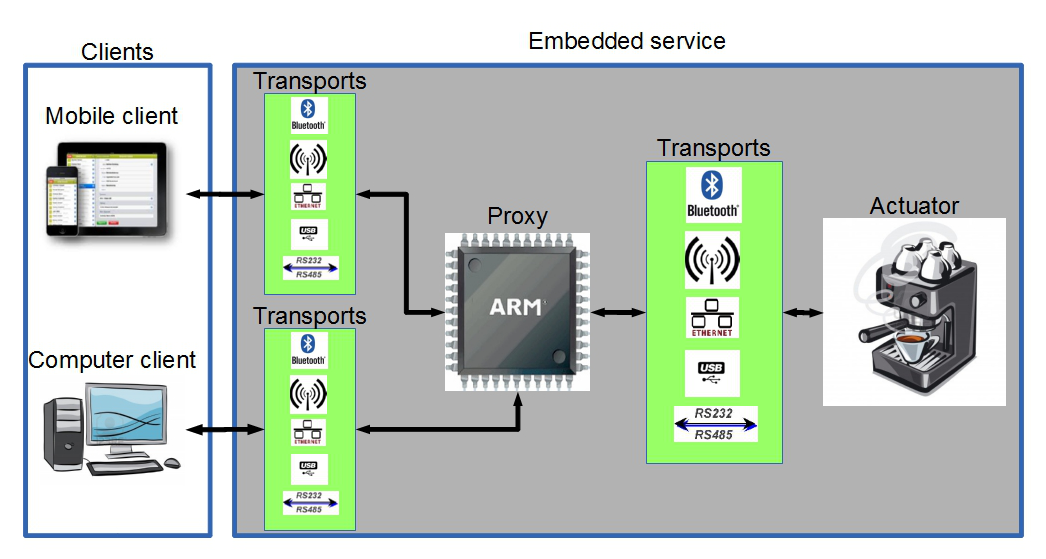
\includegraphics[width=\textwidth]{../images/implementation/system_arch.png}
	\caption{General system architecture }
	\label{fig:general_system_arch}
 \end{figure}
\end{center}

This is a traditional client-server approach where clients ( mobile or desktop)
send the requests to the server( Proxy embedded device) over some network and
physical transport( Bluetooth, various radio frequency connections, ethernet,
USB, serial line, \ldots). Proxy server is connected to the controlled device 
(marked on the figure as Actuator), which is the coffee machine in this example
application.

There can be different clients and proxy can control and monitor various
devices, but connection scheme 
\(
{Client}\leftrightarrow{Transport}\leftrightarrow{Proxy}\leftrightarrow{Transport}\leftrightarrow{{Controlled~
or~monitored~device}} \)  is essential.

In this application mobile clients are connected through Bluetooth wireless. 
Each client may be connected using supported by the proxy device transport.
The proxy is connected to coffee machine by wires and serial line. 

Next section covers the internals of Proxy device.

